\chapter{System Identification}

\textbf{System name:} Helicopter azimuth \\

\textbf{List of files:} 

\begin{tabular}{ |c|c| }
    \hline
    data\_\*.mat             & measured data \\
    main.m                  & load parameters, open models, plot input data \\
    model.slx               & model \\
    ident\_session.sid      & model identification session \\
    estimation\_session.mat & estimation session \\
    \hline
\end{tabular} \\

\section{System analysis and generation I/O data}\label{sec:data}

The following Simulink model was used to measure the data
\ref{fig:data_measure}

\begin{figure}[htb!]
    \centering
    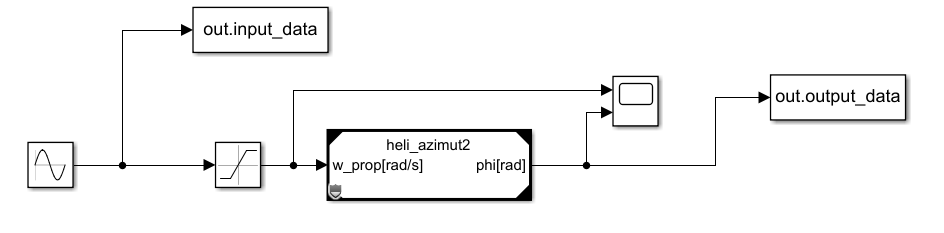
\includegraphics[width=0.8\textwidth]{data_measure.png}
    \caption{Simulink model for data measurement}
    \label{fig:data_measure}
\end{figure}

3 types of input data were used: step, impulse, random numbers responses.
\ref{fig:ident_data_1}.

\begin{figure}[htb!]
    \centering
    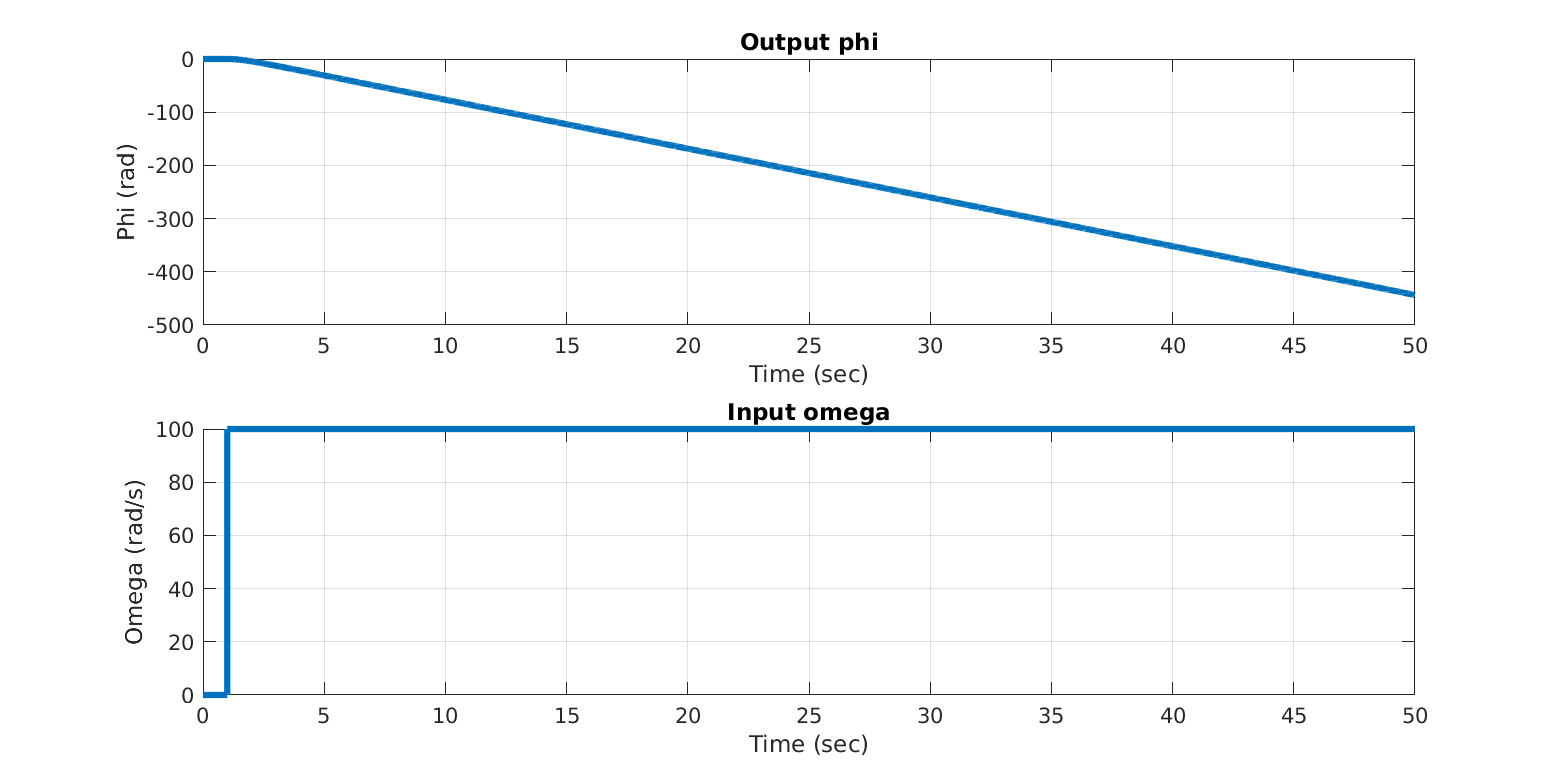
\includegraphics[width=1\textwidth]{ident_step.png}
    \caption{Simulink model for data measurement}
    \label{fig:ident_data_1}
\end{figure}
\begin{figure}[htb!]
    \centering
    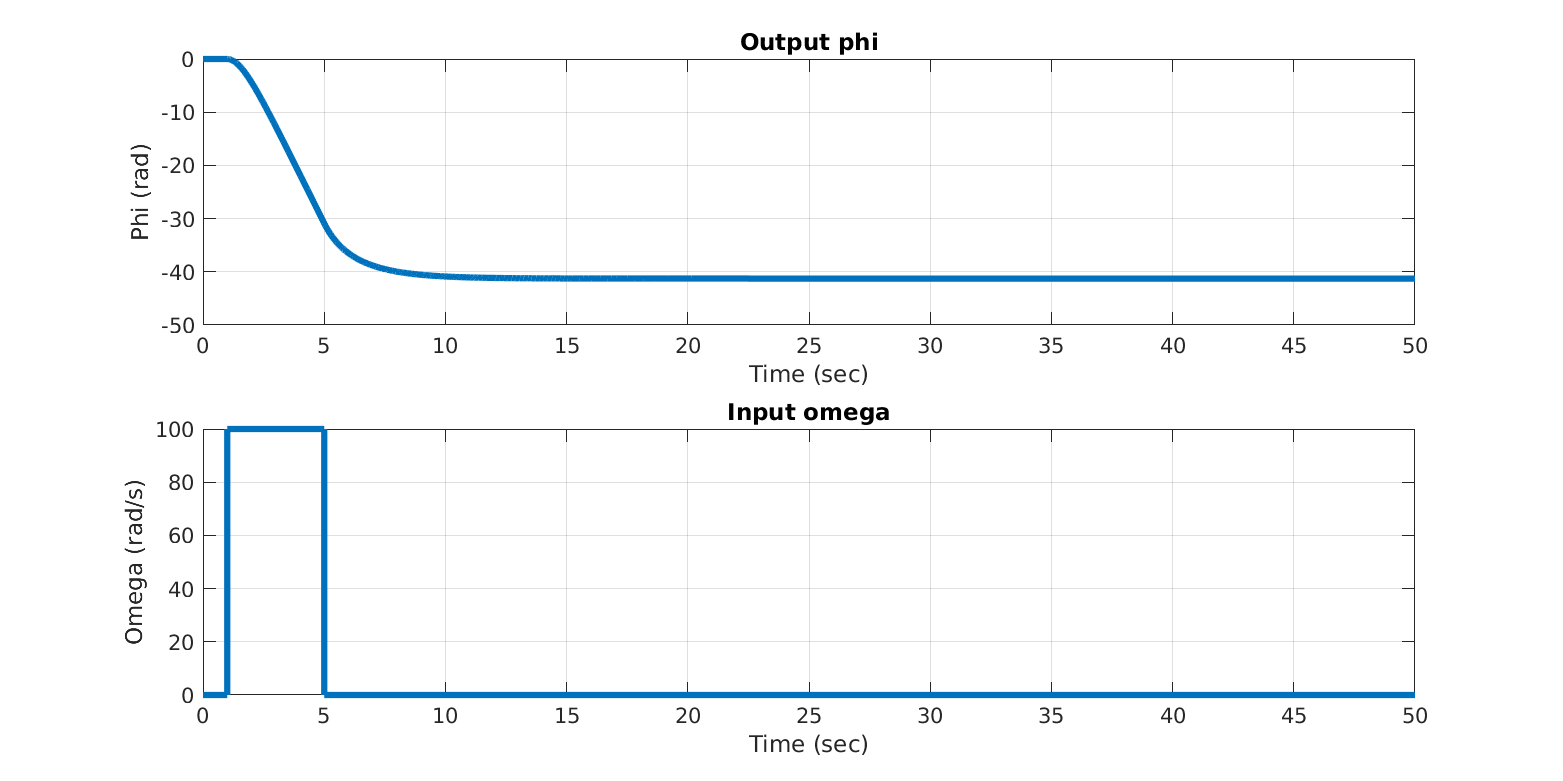
\includegraphics[width=1\textwidth]{ident_imp.png}
    \caption{Simulink model for data measurement}
    \label{fig:ident_data_2}
\end{figure}
\begin{figure}[htb!]
    \centering
    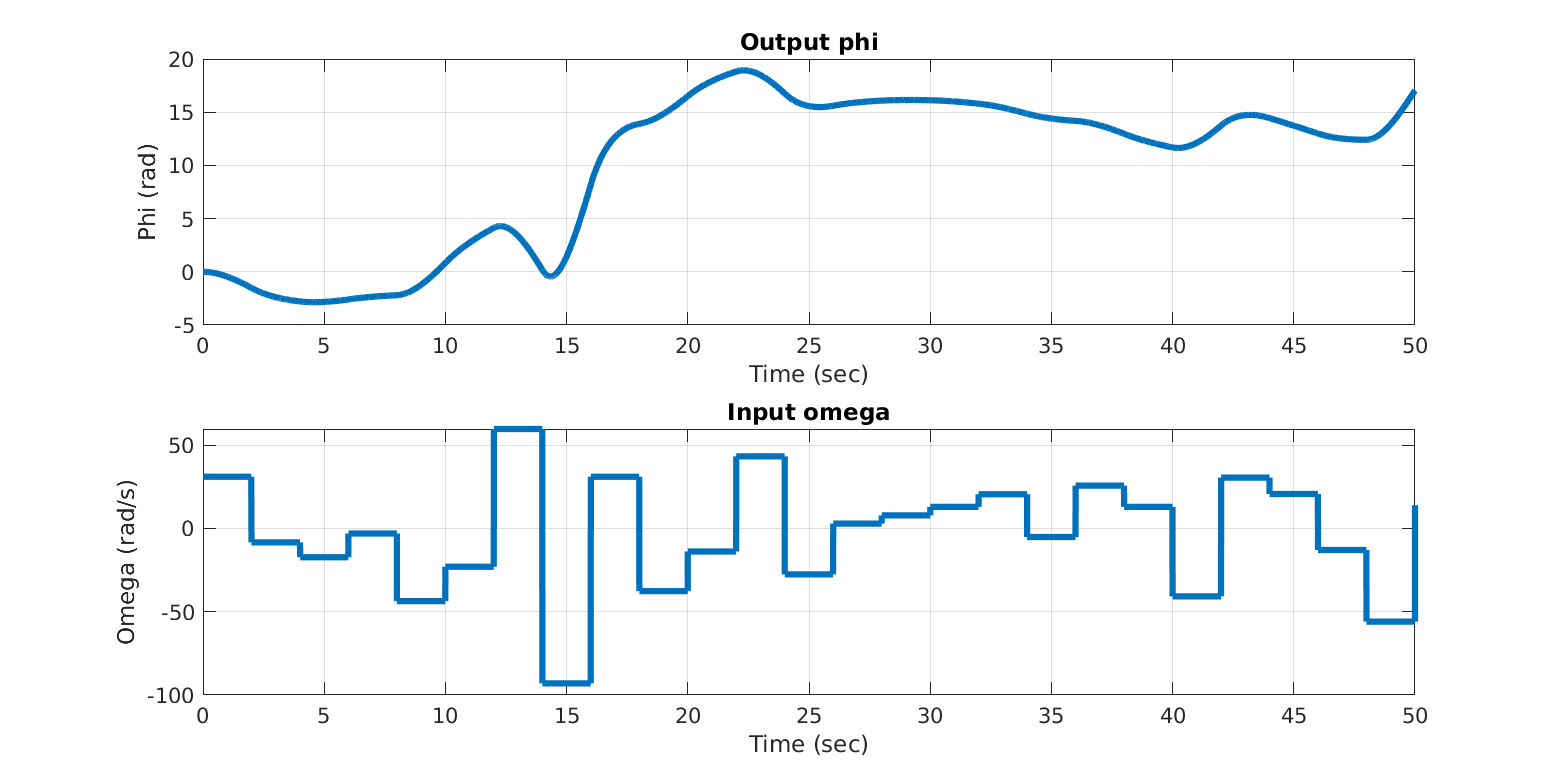
\includegraphics[width=1\textwidth]{ident_random.png}
    \caption{Simulink model for data measurement}
    \label{fig:ident_data_3}
\end{figure}

\section{Model description}

\begin{tabular}{ |c|c| }
    \hline
    $a$                 & Side length of flat plate perpendicular to flow [$m$]\\
    $\theta$            & Turn angle [$rad$]\\
    $m$                 & Mass [$kg$]\\
    $\omega$            & Angular velocity of propeller [$rad/s$]\\
    $L$                 & Length [$m$]\\
    $I$                 & Moment of inertia [$kg/m^2$]\\
    $b$                 & Friction coefficient [-]\\
    $C_x \approx 1.15$  & Drag coefficient [-]\\
    $\rho \approx 1.2$  & Mass density of the fluid [$kg/m^3$]\\
    $A$                 & Propeller area [$m^2$]\\
    $S = a^2$           & Area of flat plate [$m^2$] \\
    \hline
\end{tabular} \\

\begin{figure}[htb!]
    \centering
    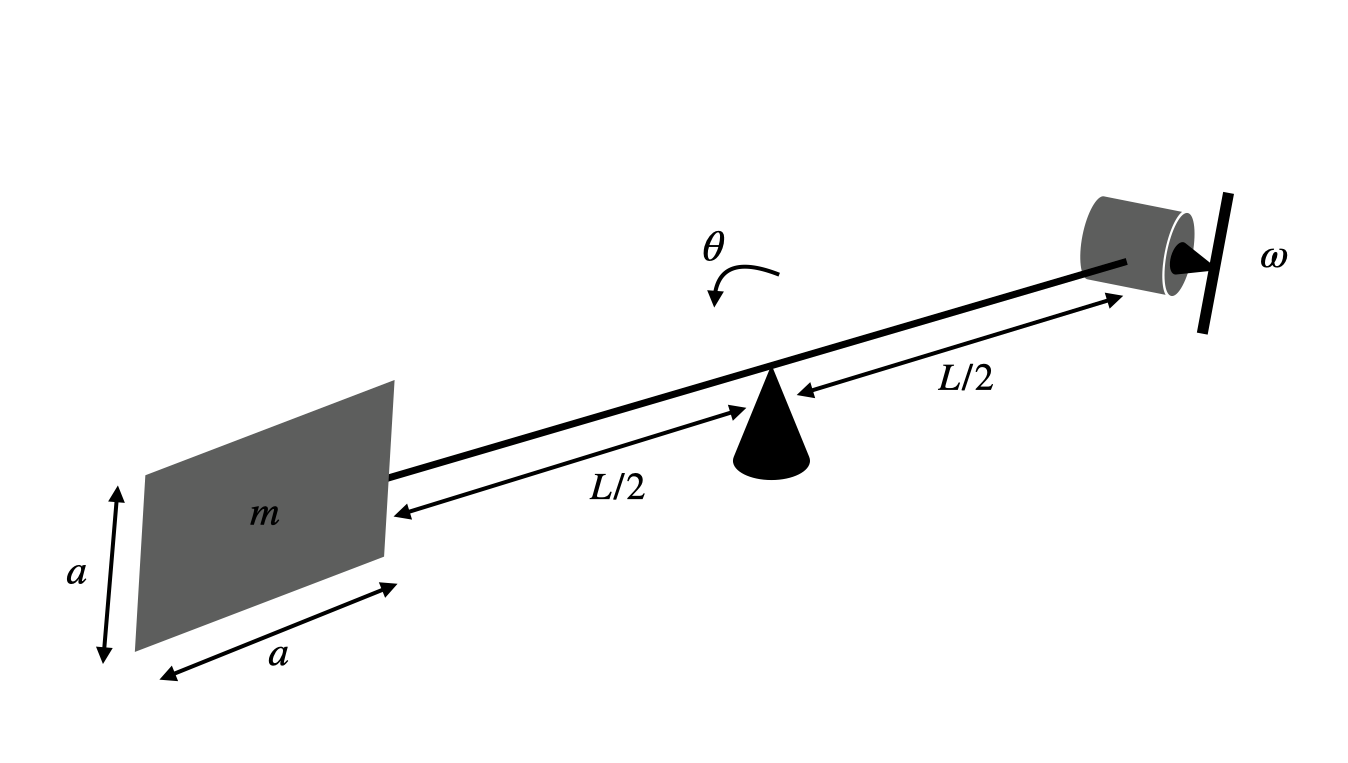
\includegraphics[width=0.6\textwidth]{ident_model.png}
    \caption{Model helicopter azimuth}
    \label{fig:ident_model}
\end{figure}
Math model of helicopter azimuth described by equation \ref{math_model_eq}.

\begin{equation}
    I\ddot{\theta} = M_{prop} - (M_f + M_d)
\end{equation}

$M_d = \frac{1}{2} C_x \rho S \frac{L}{2}\dot{\theta}^2$ -  
drag equation.
$M_f =  b\dot{\theta} + F_c \cdot \text{sign}(\dot{\theta})$ - friction momentum.
$M_p = \frac{\rho AL}{4}\omega^2$ - momentum from propeller thrust.

\begin{equation}\label{math_model_eq}
    I\ddot{\theta} = \frac{\rho AL}{4}\omega^2 - b\dot{\theta} - F_c \cdot \text{sign}(\dot{\theta})
    - \frac{1}{2}C_x \rho S \frac{L}{2}\dot{\theta}^2 
\end{equation}

Parameters to estimation:
$p_0 = \frac{AL}{I}$, $p_1 = \frac{b}{I}$, $p_2 = \frac{SL}{I}$, $p_3 =
\frac{F_c}{I}$

Simulink model represented in following diagram
\ref{fig:ident_model_simulink_full}.
\begin{figure}[htb!]
    \centering
    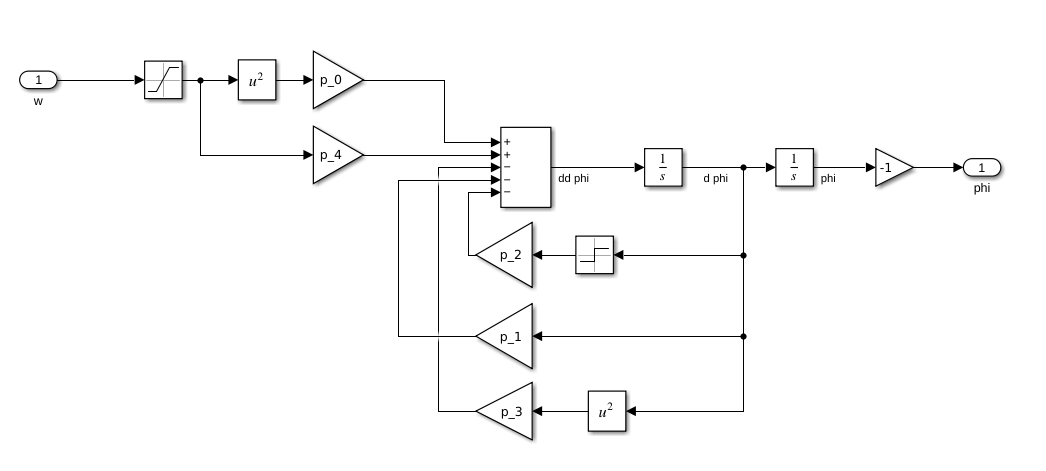
\includegraphics[width=0.8\textwidth]{identification_model.png}
    \caption{Simulink model of helicopter azimuth}
    \label{fig:identification_model}
\end{figure}

\begin{figure}[htb!]
    \centering
    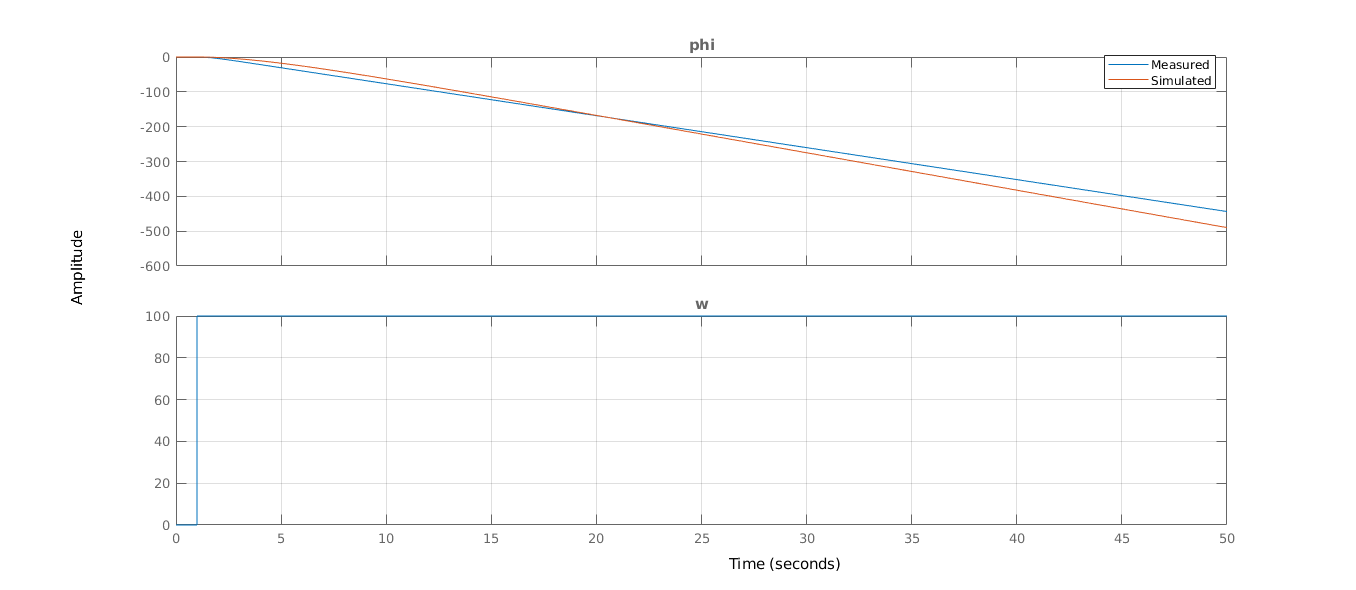
\includegraphics[width=1\textwidth]{ident_est_step.png}
    \caption{Measured and estimated response on step input}
    \label{fig:est_step}
\end{figure}
\begin{figure}[htb!]
    \centering
    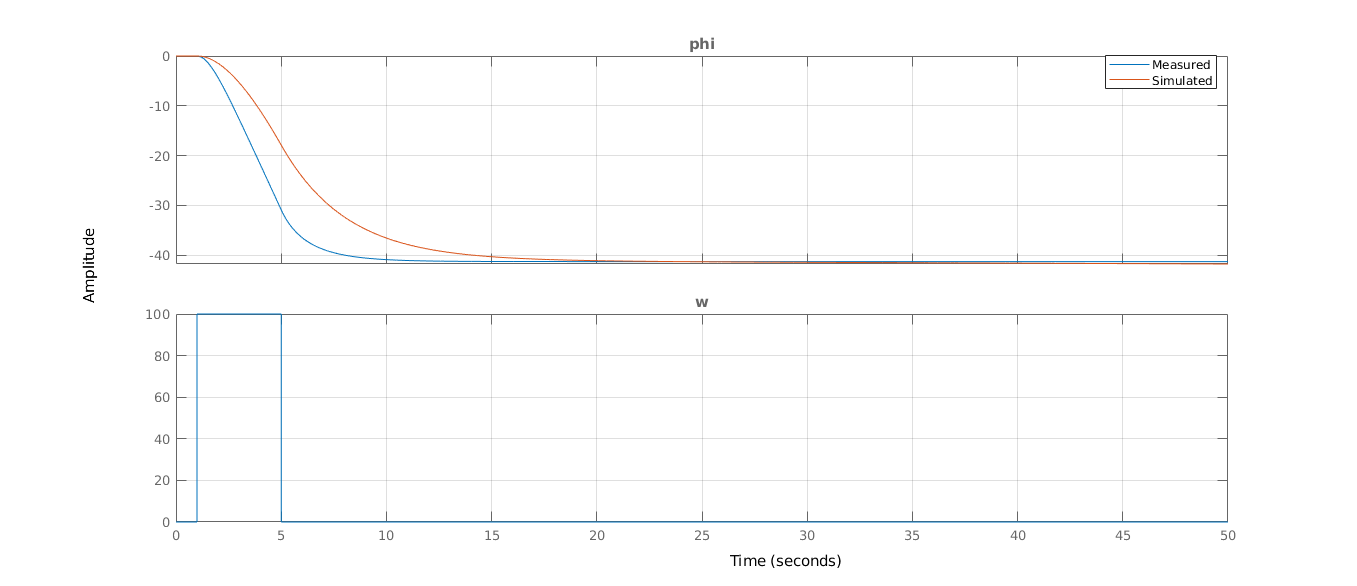
\includegraphics[width=1\textwidth]{ident_est_imp.png}
    \caption{Measured and estimated response on impulse input}
    \label{fig:est_imp}
\end{figure}
\begin{figure}[htb!]
    \centering
    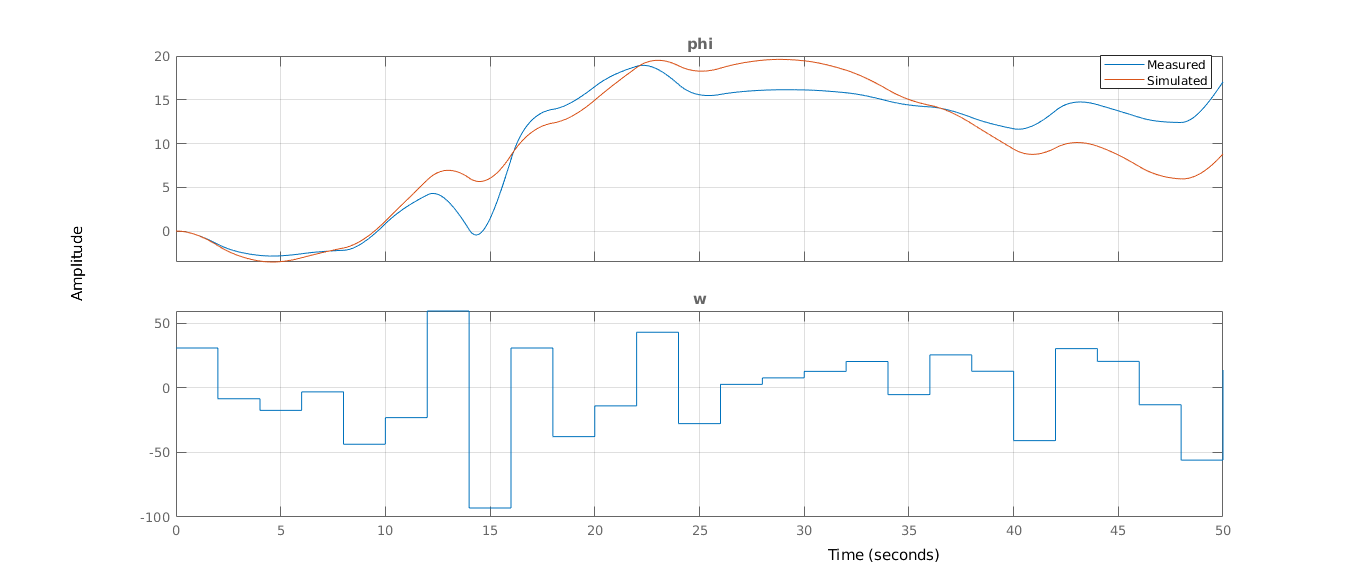
\includegraphics[width=1\textwidth]{ident_est_random.png}
    \caption{Measured and estimated response on random input}
    \label{fig:est_random}
\end{figure}

\newpage
\section{Parameter estimation}

The results are saved and can be checked in \textbf{estimation\_session.mat}.
The best courses that were achieved are shown in the graphs
\ref{fig:est_step}, \ref{fig:est_imp} and \ref{fig:est_random}.   


\section{Feed-forward}

\newpage
\section{System Identification (Black-box)}
Black-box model was developed using System Identification toolbox. As
working signals, measurements from section was used \ref{sec:data}.


\newpage
\section{Evaluation of the whole task and conclusion}
The gray box model seems correct, but the estimated parameters do not match
the reference signals well. Estimation was performed responsibly, but the
expected results were not achieved. A possible cause may be some effects
that were not taken into account in the model. The Blackbox model similarly
corresponds to the reference signals quite inaccurately. A possible reason
is the large nonlinearities and effects that were not taken into account in
the models.
